
\documentclass{beamer}
\usetheme{Electromagnetism}
\usepackage{Electromagnetism}
\graphicspath{{pictures/}}
% -------------------------------------- Grid
%-------------------------------------------------------
\makeatletter
\def\grd@save@target#1{%
  \def\grd@target{#1}}
\def\grd@save@start#1{%
  \def\grd@start{#1}}
\tikzset{
  grid with coordinates/.style={
    to path={%
      \pgfextra{%
        \edef\grd@@target{(\tikztotarget)}%
        \tikz@scan@one@point\grd@save@target\grd@@target\relax
        \edef\grd@@start{(\tikztostart)}%
        \tikz@scan@one@point\grd@save@start\grd@@start\relax
        \draw[minor help lines] (\tikztostart) grid (\tikztotarget);
        \draw[major help lines] (\tikztostart) grid (\tikztotarget);
        \grd@start
        \pgfmathsetmacro{\grd@xa}{\the\pgf@x/1cm}
        \pgfmathsetmacro{\grd@ya}{\the\pgf@y/1cm}
        \grd@target
        \pgfmathsetmacro{\grd@xb}{\the\pgf@x/1cm}
        \pgfmathsetmacro{\grd@yb}{\the\pgf@y/1cm}
        \pgfmathsetmacro{\grd@xc}{\grd@xa + \pgfkeysvalueof{/tikz/grid with coordinates/major step}}
        \pgfmathsetmacro{\grd@yc}{\grd@ya + \pgfkeysvalueof{/tikz/grid with coordinates/major step}}
        \foreach \x in {\grd@xa,\grd@xc,...,\grd@xb}
        \node[anchor=north] at (\x,\grd@ya) {\pgfmathprintnumber{\x}};
        \foreach \y in {\grd@ya,\grd@yc,...,\grd@yb}
        \node[anchor=east] at (\grd@xa,\y) {\pgfmathprintnumber{\y}};
      }
    }
  },
  minor help lines/.style={
    help lines,
    step=\pgfkeysvalueof{/tikz/grid with coordinates/minor step}
  },
  major help lines/.style={
    help lines,
    line width= 0.5pt,
    step=\pgfkeysvalueof{/tikz/grid with coordinates/major step}
  },
  grid with coordinates/.cd,
  minor step/.initial=.2,
  major step/.initial=1,
  major line width/.initial=2pt,
}
\makeatother
\usepackage{cancel}

\usetikzlibrary{decorations.pathmorphing,
                patterns, positioning,
                quotes,
                shapes.geometric}
\begin{document}



% ============================== Слайд ## ===================================
\begin{frame}{Хвильове рівняння}{}
	\begin{block}{}\justifying
		Хвиля --- це процес поширення коливань в часі та в просторі.
		Хвиля характеризується деякою величиною $u$. Наприклад, у
		випадку хвилі, що поширюється вздовж ланцюжка осциляторів $u$ -- це відхилення від їхнього положення в стані рівноваги.
	\end{block}
	\begin{onlyenv}<1>
		\begin{center}
			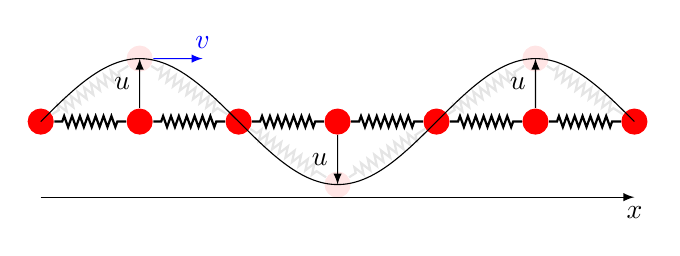
\begin{tikzpicture}[>=latex, scale=0.8,
					bord/.style = {rectangle, fill=blue,
							pattern = north east lines,
							minimum width=5mm, minimum height=25mm,
							yshift=15mm,
							node contents={}},
					mass/.style = {circle, minimum width=2*0.05, fill=red},
					spring/.style = {thick,decorate,decoration={zigzag,
									segment length = 1mm,
									amplitude=0.7mm,
									pre length=1mm, post length=1mm}
						},
				]

				% Начальная точка
				\coordinate (m0) at (0,0);

				% Создаём узлы и соединяем их
				\foreach \i [evaluate=\i as \x using \i*pi/2, evaluate=\i as \y using sin(deg(\x)), count=\j from -1] in {0,...,6} {
						% Создаём массы на синусоиде
						\node[mass] (m\i) at (\x, 0) {};
						\node[mass, opacity=0.1] (um\i) at (\x, \y) {};

						% Рисуем стрелки вверх/вниз для нечётных узлов
						\ifodd\i
							\draw[->] (m\i) --++(0, {(-1)^((\i-1)/2)}) node[left, pos=0.5] {$u$};
						\fi

						% Соединяем соседние узлы пружинами
						\ifnum\i>0
							\draw[spring, opacity=0.1] (um\j) -- (um\i);
							\draw[spring] (m\j) -- (m\i);
						\fi

						\ifnum\i=1
							\draw[->, blue] (um\i) --++(1, 0) node[above] {$\vect{v}$};
						\fi
					}

				% Рисуем синусоиду
				\draw[samples=100, domain=0:6*pi/2, smooth] plot(\x, {sin(deg(\x))});
				\draw[->] (0, -1.2) -- (6*pi/2, -1.2) node[below] {$x$};

			\end{tikzpicture}
		\end{center}
	\end{onlyenv}

	\begin{block}{}\justifying
		Диференціальне рівняння, яке описує процес поширення хвилі:
		\begin{equation*}
			\frac{\partial^2 u}{\partial x^2} + \frac{\partial^2 u}{\partial y^2} + \frac{\partial^2 u}{\partial z^2}= \frac1{v^2}\pparttime{u}
		\end{equation*}
		і називається \alert{хвильовим рівнянням}.
	\end{block}
	\begin{alertblock}{}\centering
		Якщо закони фізики приводять до такого типу рівняння --- то ці закони описують процес поширення хвиль.
	\end{alertblock}
	\begin{onlyenv}<2>
		\begin{block}{}
			Загальним розв'язком такого рівняння є функція:
			\begin{equation*}
				u = f(\vect{r} - \vect{v}t) + g(\vect{r} + \vect{v}t).
			\end{equation*}
		\end{block}
	\end{onlyenv}

\end{frame}
% ===========================================================================

\end{document}